\chapter{Implementatie}

\section{Checkin}

Als de gebruiker het lab binnen loopt, moet hij eerst inchecken. Om dat mogelijk te maken is een apart pagina gemaakt. Deze pagina is in 
Figuur \ref{fig:checkinoutview} te zien. Het bestaat uit 3 hoofdcomponenten: het welkomsbericht, de checkin knoppen en de checkout tabel.

\begin{figure}[Hh]
	\centering
	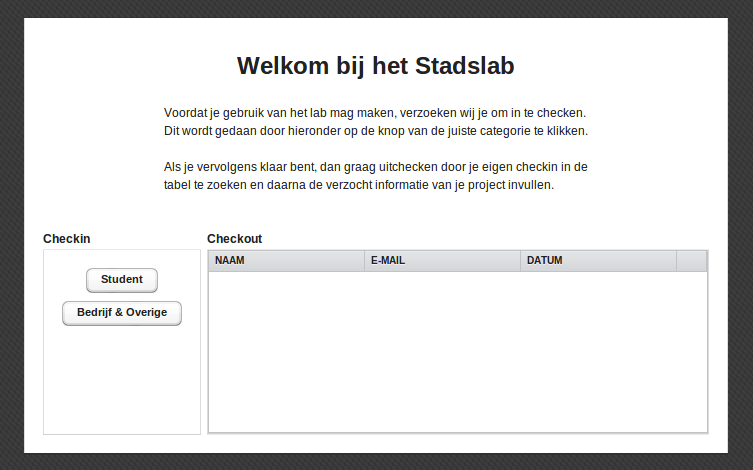
\includegraphics[width=\textwidth]{Images/checkinoutview2.png}
	\caption{Venster waar kan worden ingecheckt en uitgecheckt}
	\label{fig:checkinoutview}
\end{figure}

Het welkomsbericht bestaat uit een korte stuk tekst waarin uitgelegd wordt wat de bedoeling van deze pagina is. \\
Daaronder staan de checkin knoppen. Gebruikers horen de knop te kiezen dat bij hun past, als student of bedrijf/overige zijnde.\\ 

\subsection{Student}

Als een student in wilt checken, dan krijgt de student een venster te zien als weergegeven in Figuur \ref{fig:checkin-student}. Hierbij wordt persoonlijk informatie van de student gevraagd dat door de beheerders gebruikt wordt om bijvoorbeeld kosten te declareren bij de corresponderende instituut. Er wordt verder ook gevraagd met welke apparaten de student zal gaan werken. Hierdoor kunnen de beheerders een overzicht krijgen over welke apparaten de populairste zijn. Verder is er validatie ingebouwd om te zorgen dat alle velden ingevuld zijn, als afgebeeld in Figuur \ref{fig:checkin-student-error}. \\

\begin{figure}[Hh]
	\centering
	\subfigure[Checkin met ingevuld gegevens]{
		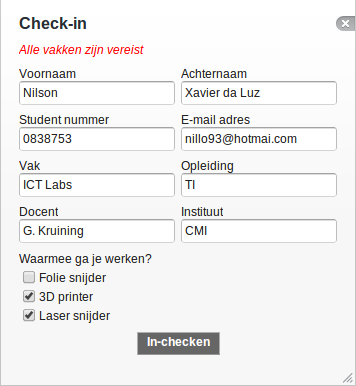
\includegraphics[width=175px, height=225px]{Images/checkin-student.png}
		\label{fig:checkin-student}
	}
	\subfigure[Checkin met errors]{
		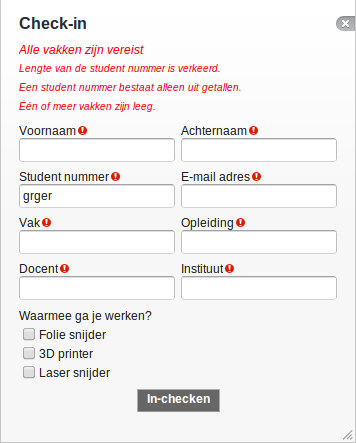
\includegraphics[width=175px, height=225px]{Images/checkin-student-error.png}
		\label{fig:checkin-student-error}
	}
	\caption{Checkin voor studenten}
\end{figure}

\subsection{Bedrijf en Overige}

Als een bedrijf of overige iemand in wilt checken dat krijgt diegene ook een eigen venster te zien. Hier wordt andere soort informatie gevraagd dat meer bij deze categorie past. Dit venster is te zien bij Figuur \ref{fig:checkin-company}. Ook hier wordt de ingevuld informatie gevalideerd om te zorgen dat alle informatie ingevuld is, dit is weergegeven in Figuur \ref{fig:checkin-company-error}. \\

\begin{figure}[Hh]
	\centering
	\subfigure[Checkin met ingevuld gegevens]{
		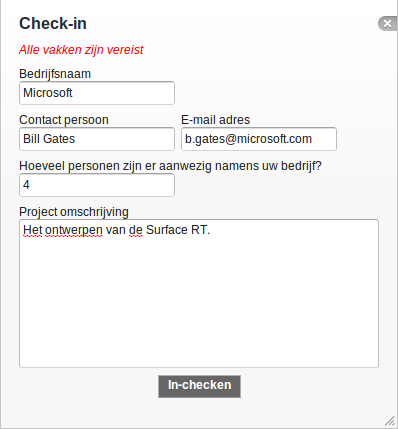
\includegraphics[width=175px, height=225px]{Images/checkin-company.png}
		\label{fig:checkin-company}
	}
	\subfigure[Checkin met errors]{
		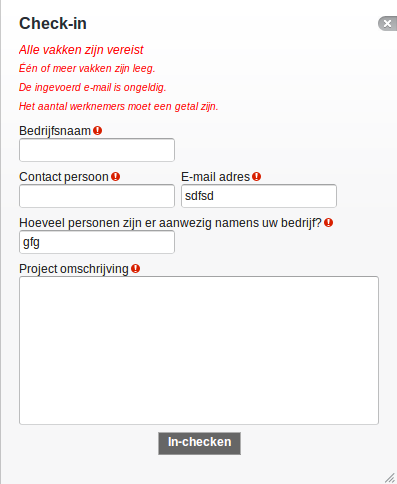
\includegraphics[width=175px, height=225px]{Images/checkin-company-error.png}
		\label{fig:checkin-company-error}
	}
	\caption{Checkin voor bedrijven}
\end{figure}

Zodra de gebruiker heeft ingecheckt, dan is de gebruiker vrij om gebruik te maken van het lab. Er komt dan een nieuwe element in de checkouts tabel te staan met de informatie van de gebruiker en een knop om uit te checken. Dit is te zien in Figuur \ref{fig:checkout-table}. \\

\begin{figure}[Hh]
	\centering
	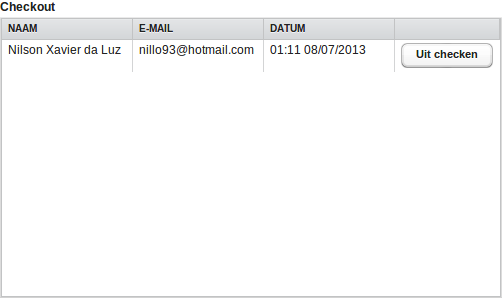
\includegraphics[width=0.65\textwidth]{Images/checkout-table.png}
	\caption{Pagina waar kan worden ingecheckt en uitgecheckt}
	\label{fig:checkout-table}
\end{figure}

\section{Checkout}

Wanneer de gebruiker klaar is en het lab wilt verlaten, wordt hij verzocht om eerste uit te checken. Dit gebeurt door zijn eigen informatie op te zoeken in de tabel en op de ``Uit checken'' knop te drukken. Er verschijnt dan een nieuwe venster om de benodigde informatie in te vullen over het project. Dit venster is weergegeven in Figuur \ref{fig:checkout-window}.

\begin{figure}[Hh]
	\centering
	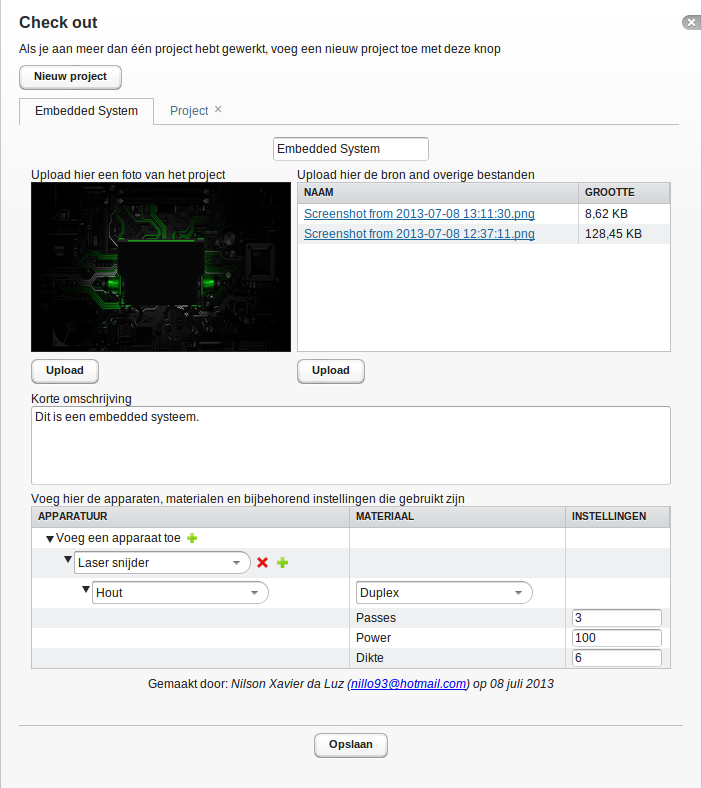
\includegraphics[width=0.65\textwidth]{Images/checkout-window.png}
	\caption{Venster waar kan worden uitgecheckt}
	\label{fig:checkout-window}
\end{figure}

Om te kunnen uitchecken wordt de volgende informatie gevraagd:

\subsection{Titel}

De titel wordt gebruikt om de project te identificeren. De titel moet uniek zijn.

\subsection{Foto}

Een foto van het project. Daarin moet duidelijk te zien zijn wat het project is.

\subsection{Bron bestanden}

Bron en overige bestanden van het project. Dit kan source code, 3D-modellen of iets anders zijn.

\subsection{Korte omschrijving}

Een korte omschrijving over wat het project is en/of doet.

\subsection{Instellingen}

Hier worden de gebruikte instellingen ingevuld van de gebruikte apparatten. Dit wordt gedaan door eerst apparaten toe te voegen, daarna materialen waaronder verschillende types te kiezen valt. Als een materiaal gekozen is, verschijnen de nodige instellingen van de gekozen apparaat en velden waar de instellingen kunnen worden ingevuld. \\

Er kunnen meerdere project worden aangemaakt voor het geval dat de gebruiker aan meerdere projecten heeft gewerkt. Dit wordt gedaan door op de ``Nieuw project'' knop bovenaan te drukken. Hierdoor wordt een nieuwe tab toegevoegd naast de tab van het bestaande project. \\
Als alles correct is ingevuld, dan wordt de checkout opgeslagen en is de gebruiker uitgecheckt.

\section{FabTool}

Het hoofdgedeelte van de webapplicatie is de FabTool, zie Figuur \ref{fig:fabtool}. Dit is waar projecten kunnen gezocht en bekeken, en waar beheerders overzicht kunnen houden over alle checkins en apparaten kunnen beheren.

\begin{figure}[Hh]
	\centering
	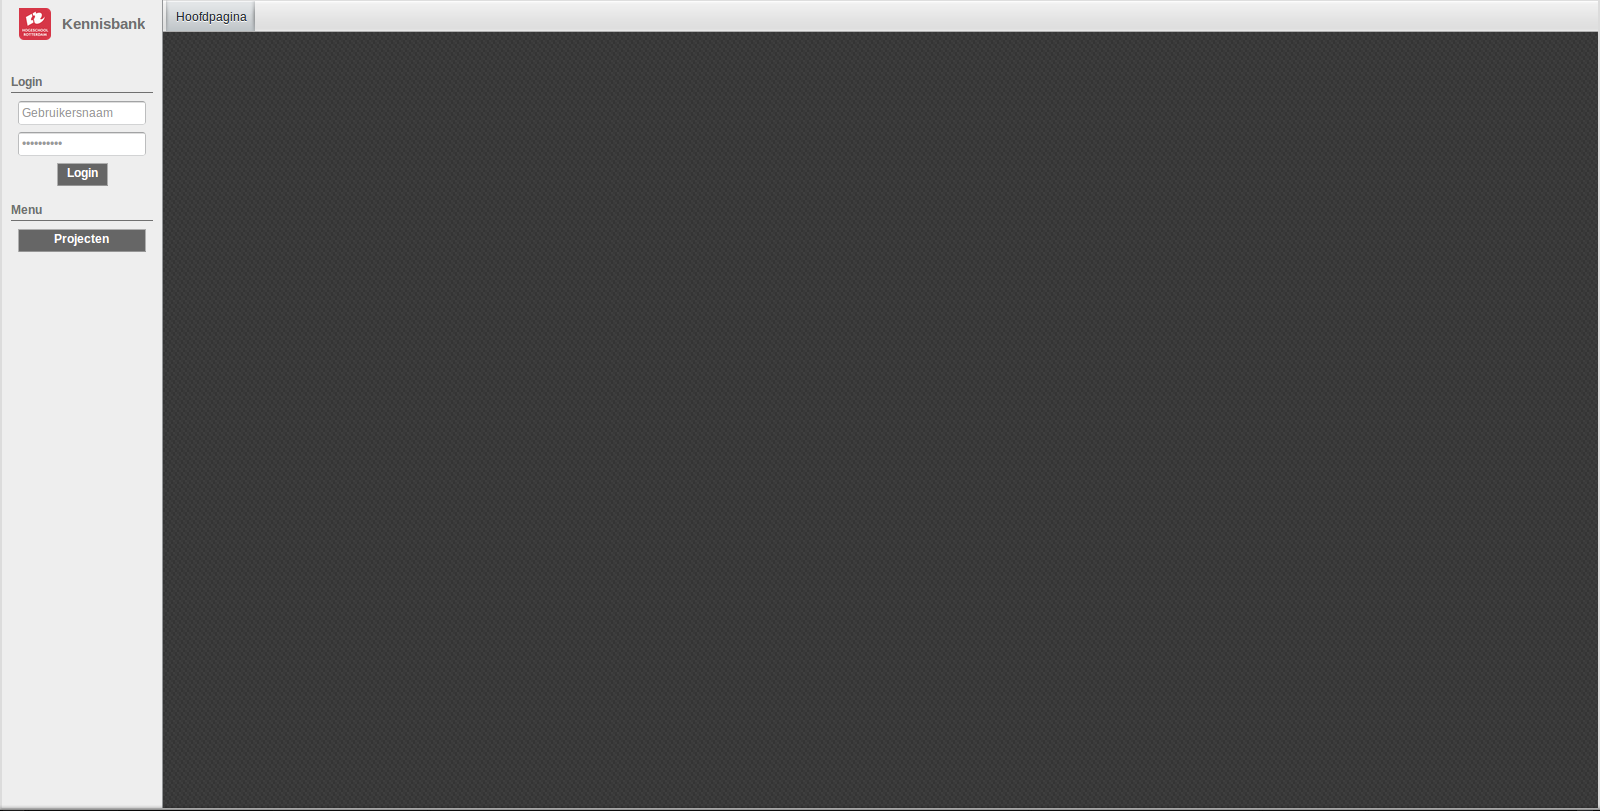
\includegraphics[width=1\textwidth]{Images/fabtool.png}
	\caption{Design van de FabTool}
	\label{fig:fabtool}
\end{figure}

\subsection{Projecten}

Een van de componenten van de FabTool zijn de projecten. Hier worden alle projecten die tot nu toe zijn gemaakt weergegeven, zoals het te zien is op Figuur \ref{fig:projects}.

\begin{figure}[Hh]
	\centering
	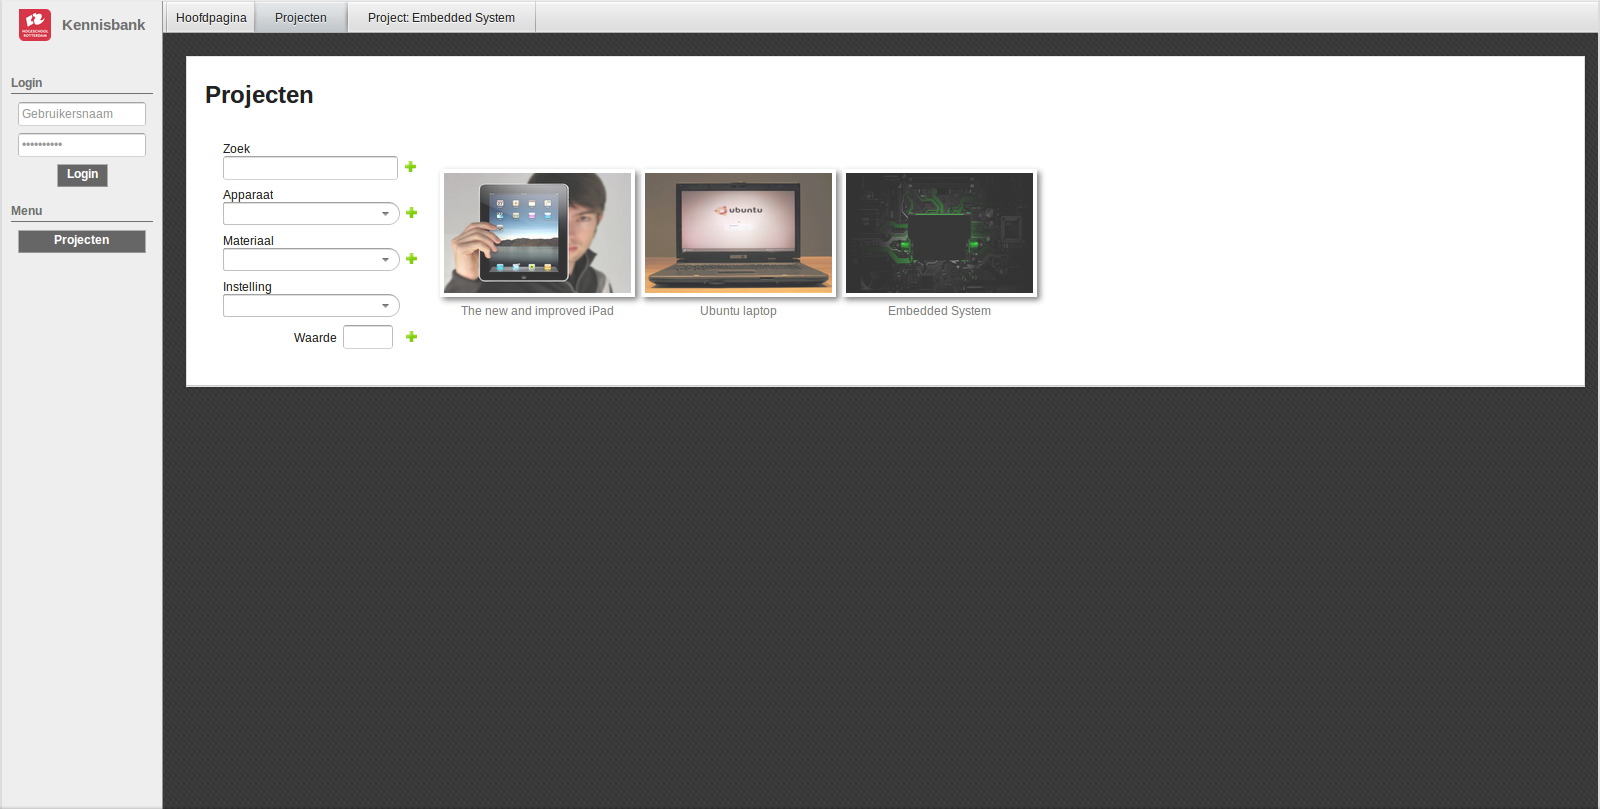
\includegraphics[width=1\textwidth]{Images/projects.png}
	\caption{Pagina waar projecten worden weergegeven}
	\label{fig:projects}
\end{figure}

Het geeft gebruikers ook de mogelijkheid om naar project te zoeken en te uit te filteren. Zoals het is weergegeven is in Figuur \ref{fig:filter-projects}, kunnen project op meerdere categori\"en worden gefilterd. Ze kunnen per soort apparaat, materiaal en instelling worden gezocht. Ook is het mogelijk om naar tekst te worden gezocht dat voorkomt in de titel of bij de omschrijving.

\begin{figure}[Hh]
	\centering
	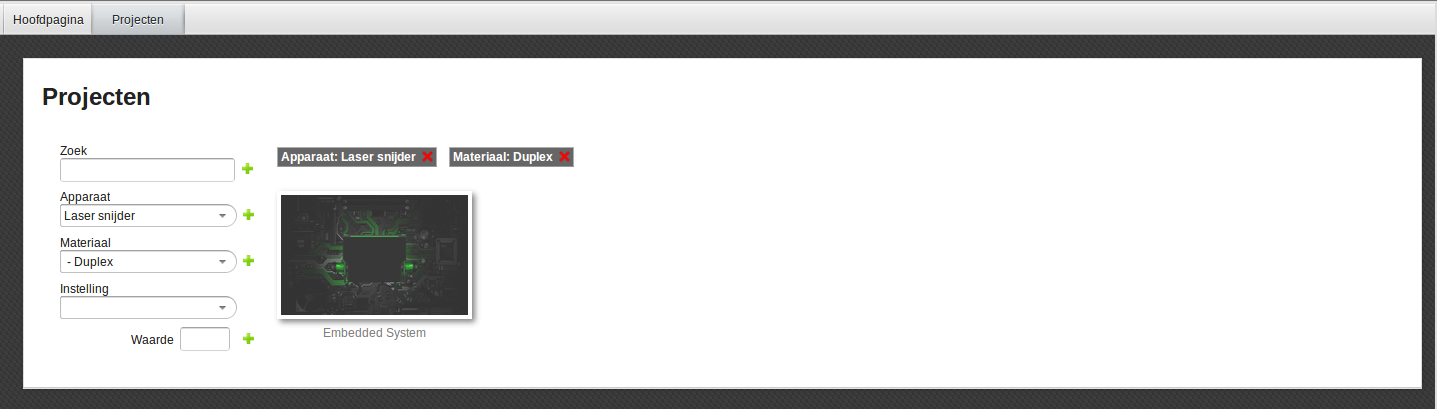
\includegraphics[width=1\textwidth]{Images/filter-projects.png}
	\caption{Projecten worden gefilterd}
	\label{fig:filter-projects}
\end{figure}

Als de gebruiker het project heeft gevonden waar hij naar zocht, kan hij erop klikken. Hierdoor verschijnt een nieuwe pagina met hetzelfde informatie dat tijdens het inchecken is ingevuld. Dit is te zien in Figuur \ref{fig:filter-projects}.

\begin{figure}[H]
	\centering
	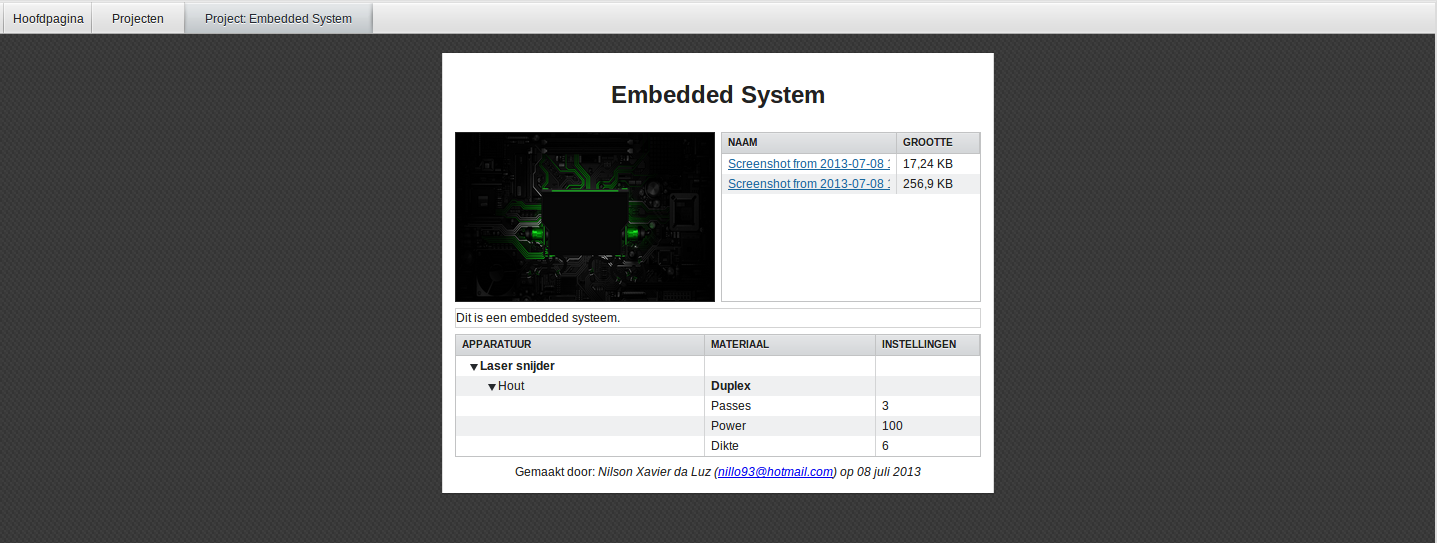
\includegraphics[width=1\textwidth]{Images/project.png}
	\caption{Gekozen project}
	\label{fig:filter-projects}
\end{figure}